\begin{center}
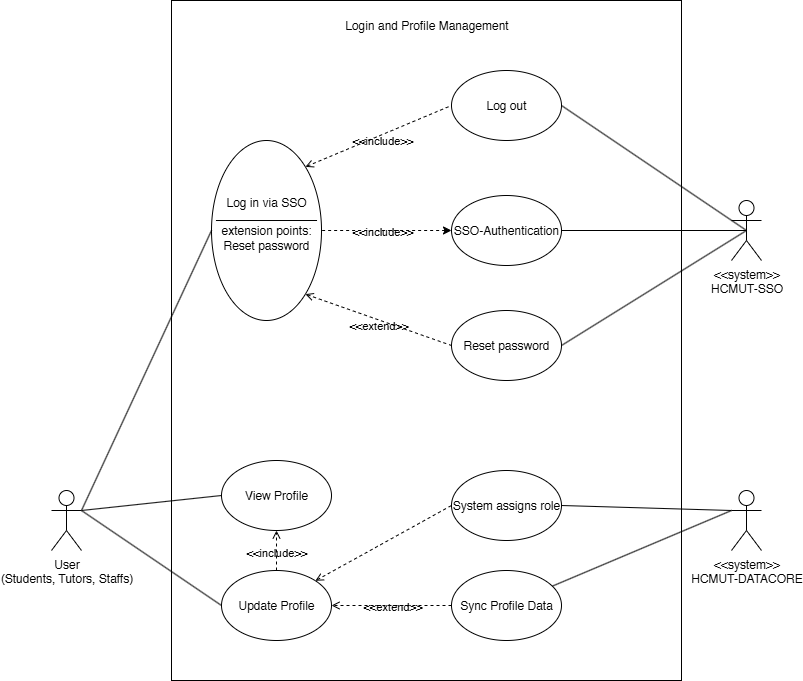
\includegraphics[width=0.9\linewidth]{images/UC-01.png}
\end{center}

\begin{center}
\textbf{Figure 2:}  Log in and Manage Profile
\end{center}  


\begin{table}[h!]
\centering
\begin{tabular}{|p{3cm}|p{11cm}|}
\hline
\textbf{Use-case ID} & UC-01a \\
\hline
\textbf{Use-case name} & Login via SSO \\
\hline
\textbf{Use-case overview} & To allow students, tutors, and staff to log in securely via HCMUT\_SSO with role assignment handled by the system. \\
\hline
\textbf{Actors} & User (Students, Tutors, Staff), HCMUT\_SSO, System \\
\hline
\textbf{Preconditions} & 
1. User has valid SSO credentials. \newline
2. HCMUT\_SSO service is available. \\
\hline
\textbf{Trigger} & User selects the ``Login via SSO'' option. \\
\hline
\textbf{Steps} & 
1. User initiates login via HCMUT\_SSO. \newline
2. System sends authentication request to SSO service. \newline
3. HCMUT\_SSO validates credentials. \newline
4. On success, the system fetches user data and assigns role. \newline
5. On failure, the system denies access. \\
\hline
\textbf{Postconditions} & User is authenticated and session established; role assignment is ready for system use. \\
\hline
\textbf{Alternative Flows} & 
A1: Invalid login → Access denied with error message. \newline
A2: Role update in DATACORE synced during login. \\
\hline
\textbf{Exception Flow} & 
1. SSO service unavailable → System shows maintenance/unavailable message. \newline
2. Network error → User prompted to retry login. \\
\hline
\end{tabular}
\caption{Use Case UC-01a: Login via SSO}
\end{table}


\begin{table}[h!]
\centering
\begin{tabular}{|p{3cm}|p{11cm}|}
\hline
\textbf{Use-case ID} & UC-01b \\
\hline
\textbf{Use-case name} & Profile Management \\
\hline
\textbf{Use-case overview} & To allow students and tutors to view and update their profiles, with core data synchronized from HCMUT\_DATACORE. \\
\hline
\textbf{Actors} & Student, Tutor, HCMUT\_DATACORE, System \\
\hline
\textbf{Preconditions} & 
1. User is authenticated via SSO. \newline
2. Profile data exists in DATACORE. \\
\hline
\textbf{Trigger} & User selects the ``View/Update Profile'' option. \\
\hline
\textbf{Steps} & 
1. System retrieves profile information from DATACORE. \newline
2. User views profile fields (ID, name, email, faculty, role). \newline
3. User updates non-core profile details. \newline
4. System validates and saves changes. \newline
5. System syncs updated data with DATACORE. \\
\hline
\textbf{Postconditions} & User profile is updated and synchronized with DATACORE; changes are timestamped and logged. \\
\hline
\textbf{Alternative Flows} & 
A1: DATACORE unavailable → Updates stored locally until sync resumes. \\
\hline
\textbf{Exception Flow} & 
1. Invalid update request → System rejects and shows error. \newline
2. Sync conflict with DATACORE → DATACORE treated as source of truth. \\
\hline
\end{tabular}
\caption{Use Case UC-01b: Profile Management}
\end{table}

